\documentclass[11pt,a4paper]{scrartcl}
\usepackage[T1]{fontenc}
\usepackage[utf8]{inputenc}
\usepackage[ngerman]{babel}
\usepackage{microtype}
\usepackage{lmodern}
\usepackage{amsmath}
\usepackage{amsfonts}
\usepackage{amssymb}
\usepackage{enumerate}
\usepackage{graphicx}


\begin{document}

\author{Gruppe 14\\Max-Emanuel Hoffmann\\Ralf Vogler\\Sebastian Wiesner}
\title{Verteilte und Web-Informationssysteme}
\subtitle{Blatt 08}

\maketitle

\section*{Aufgabe 1: Majority Consensus}


\section*{Aufgabe 2: Chord}
\subsection*{a) Fingertabellen}
siehe Abbildung\\
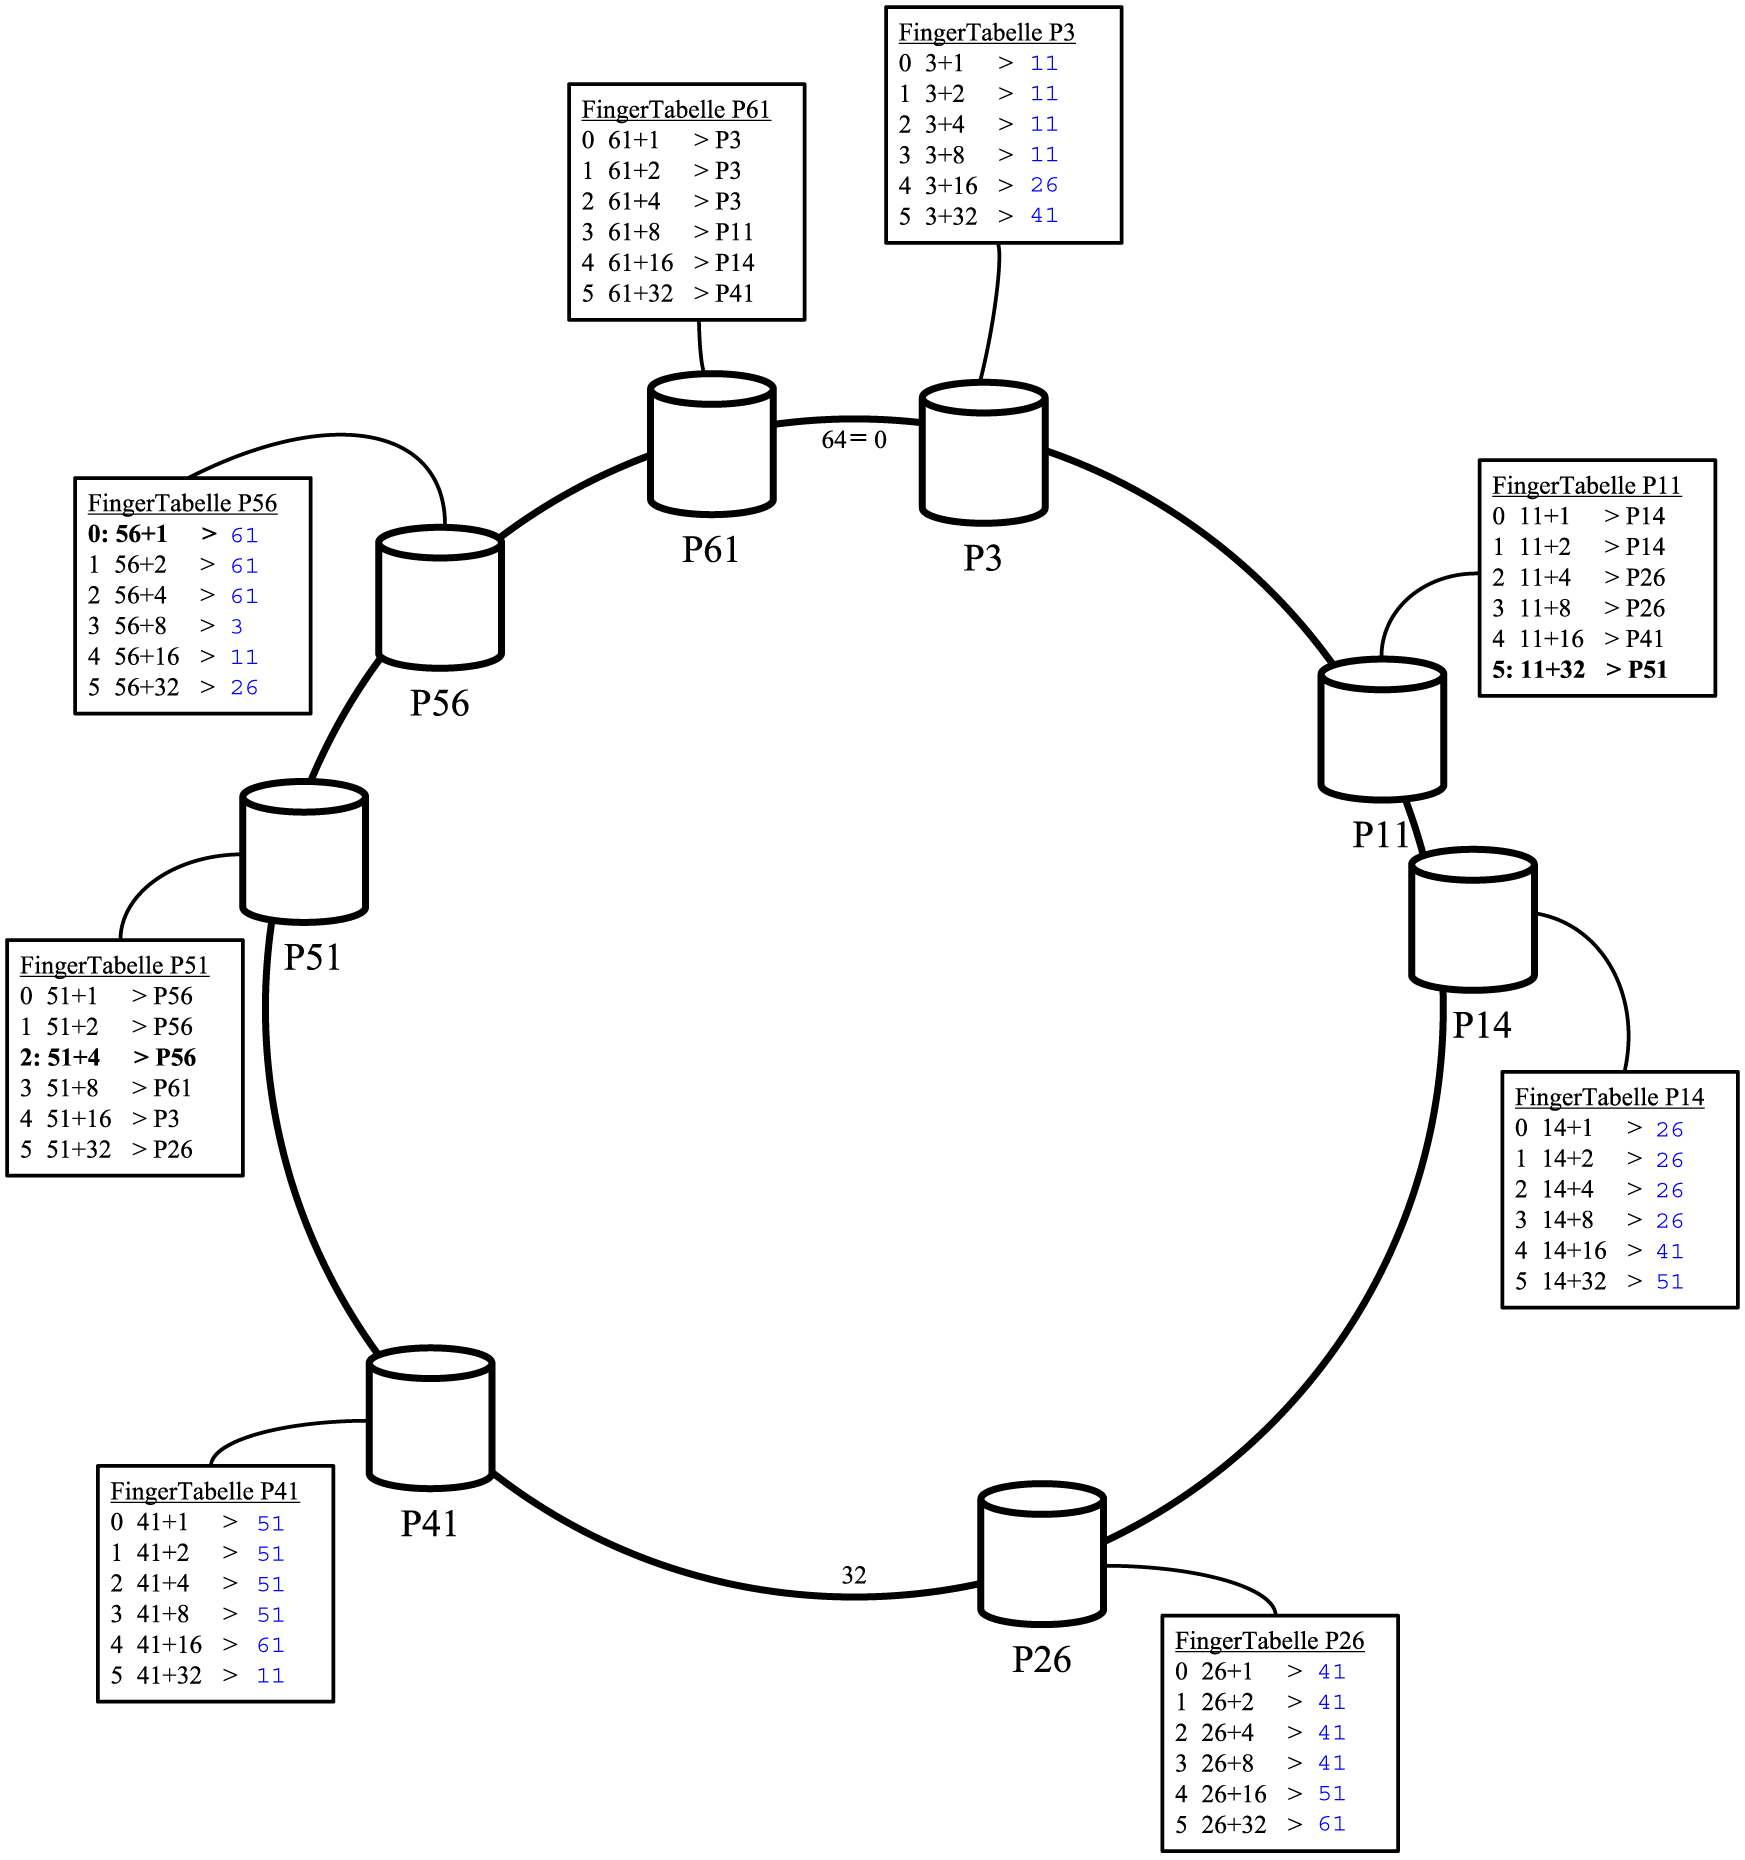
\includegraphics[width=\textwidth]{Chord1.png}


\subsection*{b) Suche in log Schritten}
Suche in Chord funktioniert wie Suche in Binärbaum -> O(log(n)).


\subsection*{c) Anfragen}
\begin{itemize}
\item{K90 von P3:} 90\%64 = 26; P3: 3+16 -> P26; P26 enthält K90
\item{K8 von P11:} P11 enthält K8
\item{K2 von P11:} 11+32 -> P51; 51+8 -> P61; 61+4 -> P3; P3 enthält K2
\item{K258 von P61:} 258\%64 = 2; 61+4 -> P3; P3 enthält K258
\end{itemize}

\subsection*{d) Neuer Peer P20}
P20 wird zwischen P14 und P26 eingefügt und danach die Fingertabellen aktualisiert.
Dabei müssen nur die Einträge überprüft werden die vorher auf P26 gezeigt haben, da dessen Zuständigkeitsbereich halbiert wurde und Sprünge nun evtl. nach P20 statt P26 gehen.

\subsection*{e) Aktualisierte Fingertabellen}
siehe Abbildung\\
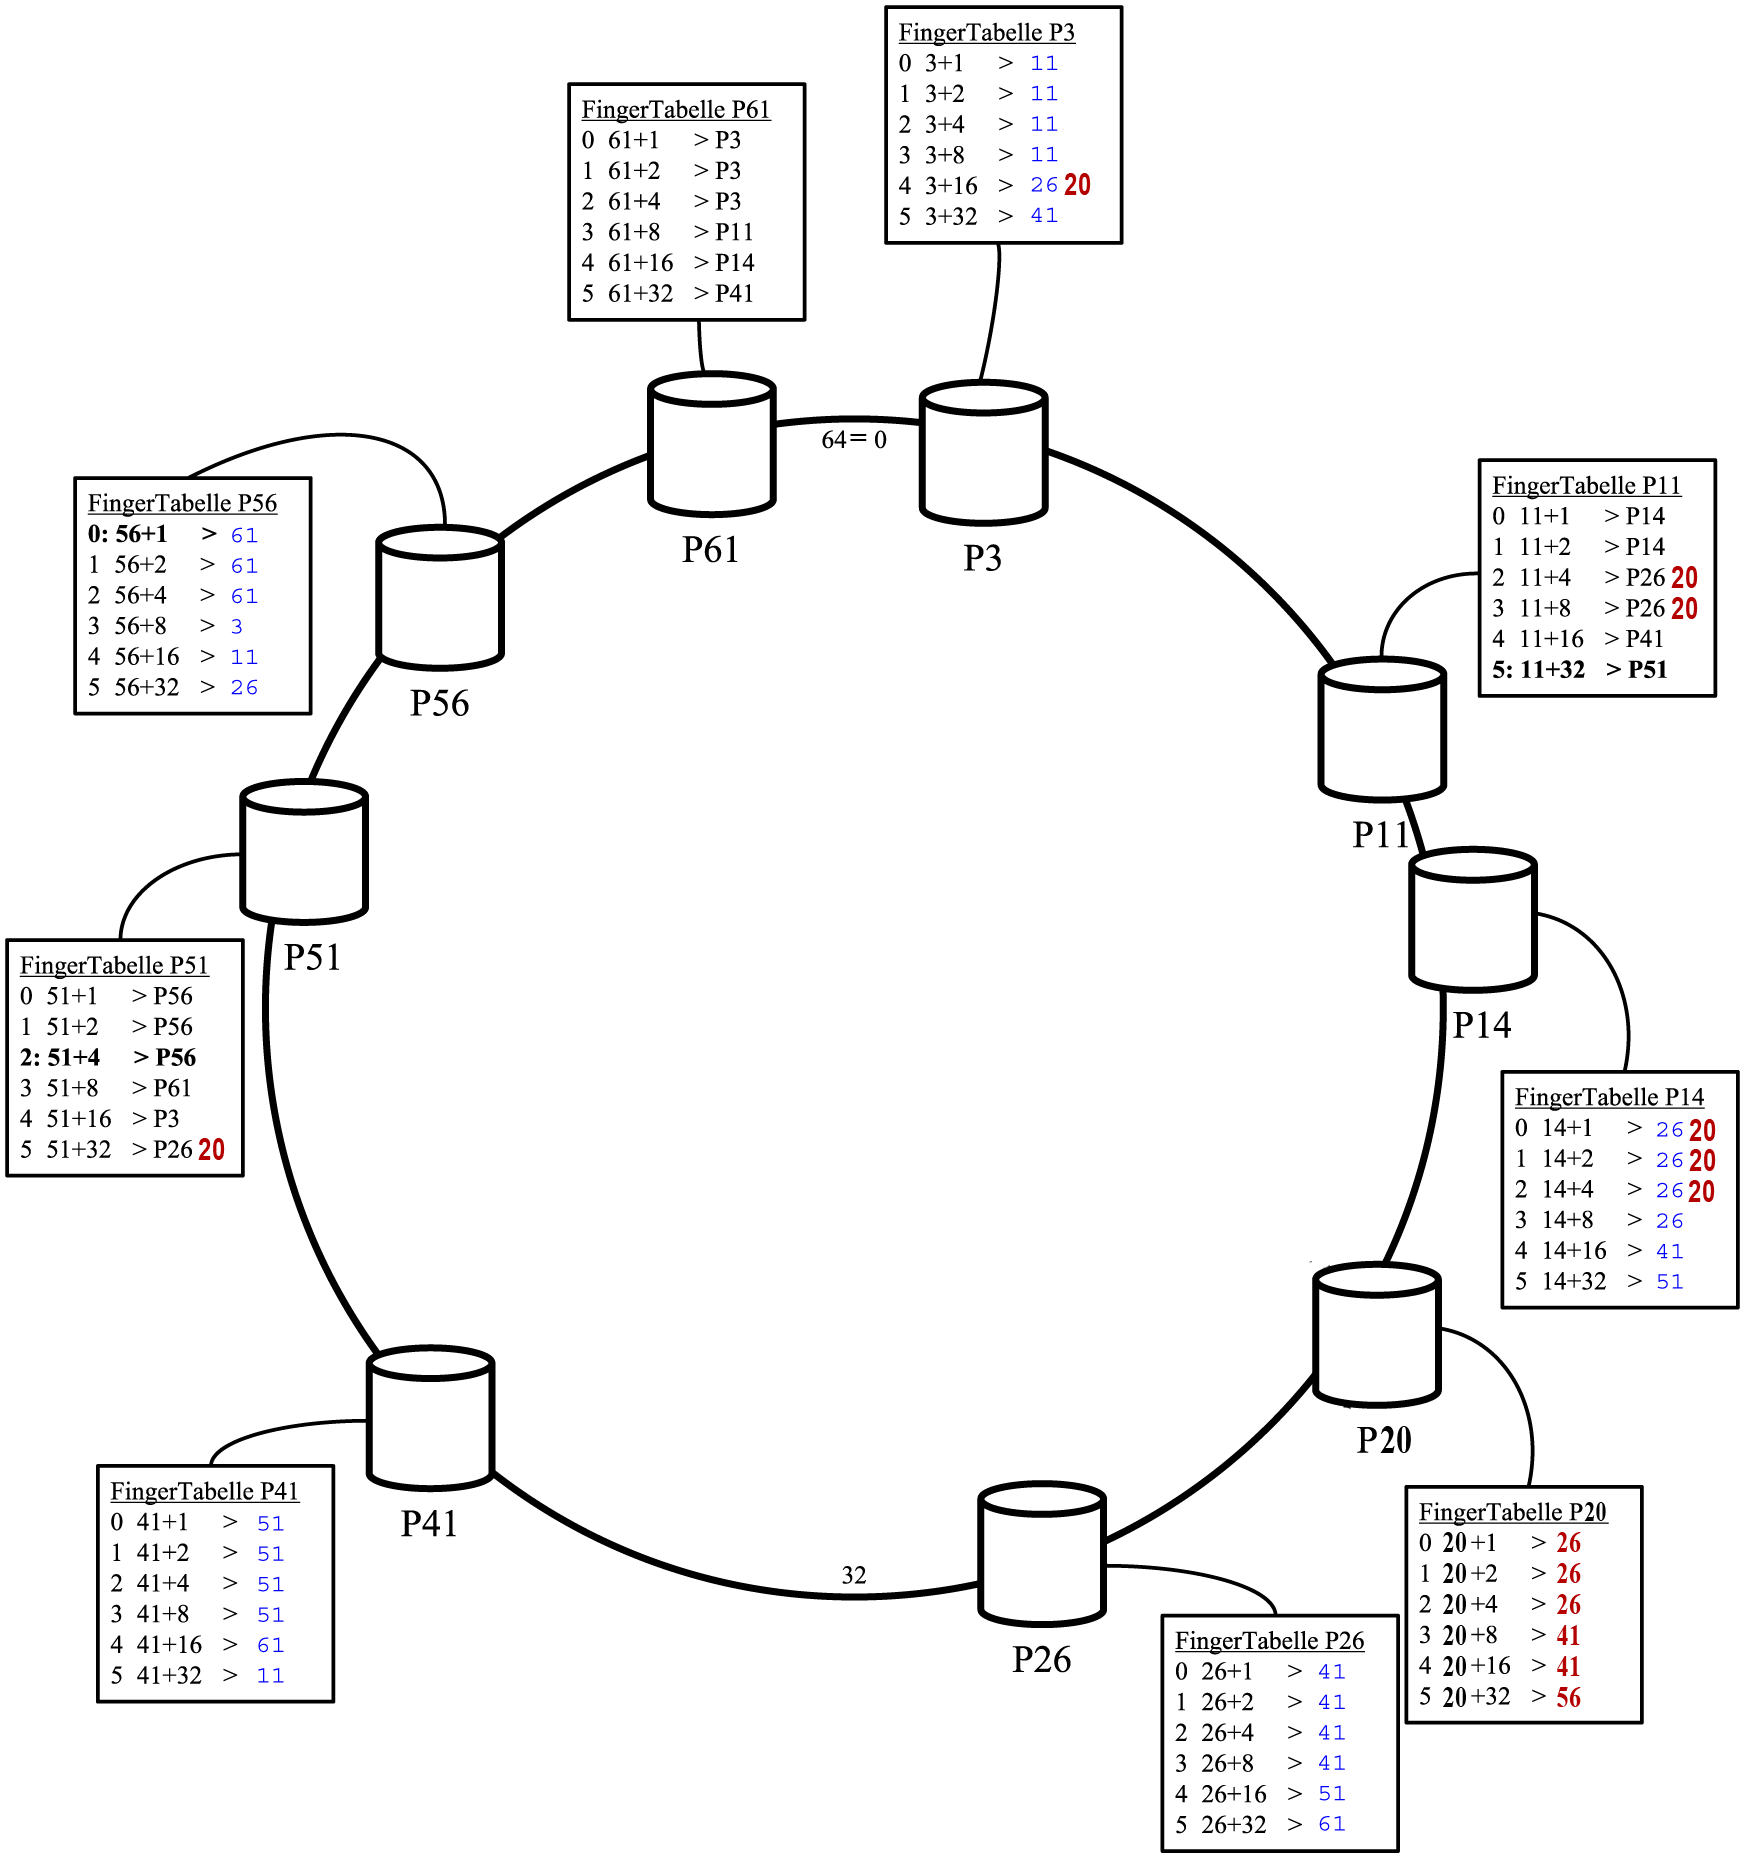
\includegraphics[width=\textwidth]{Chord2.png}


\end{document}
